\documentclass[11pt]{report}

% report format
\usepackage[utf8]{inputenc}
\usepackage[a4paper, top=3cm, bottom=3cm, left=3.5cm, right=3cm]{geometry}
\usepackage{setspace}
\onehalfspacing{}

\usepackage[hidelinks]{hyperref}
\usepackage{graphicx}
\usepackage{listings}
\usepackage{color}
\usepackage{chngcntr}
\counterwithout{footnote}{chapter}

\usepackage{biblatex}
\bibliography{main.bib}

% \usepackage{float}
% \usepackage{multirow}
% \usepackage{booktabs}
% \usepackage{tabularx}
% \usepackage{amssymb}

% some configurations for the listings package
\definecolor{codegreen}{rgb}{0,0.6,0}
\definecolor{codegray}{rgb}{0.5,0.5,0.5}
\definecolor{codepurple}{rgb}{0.58,0,0.82}
\definecolor{backcolour}{rgb}{0.95,0.95,0.92}
\lstdefinestyle{mystyle}{
    backgroundcolor=\color{backcolour},
    commentstyle=\color{codegreen},
    keywordstyle=\color{magenta},
    numberstyle=\tiny\color{codegray},
    stringstyle=\color{codepurple},
    basicstyle=\footnotesize\ttfamily,
    breakatwhitespace=false,
    breaklines=true,
    captionpos=b,
    keepspaces=true,
    % numbers=left,
    numbersep=5pt,
    showspaces=false,
    showstringspaces=false,
    showtabs=false,
}
\lstset{style=mystyle}

% actual report
\begin{document}
\pagenumbering{gobble}
\begin{titlepage}
\begin{center}

% school logo

\includegraphics[width=0.9\textwidth]{images/ntu_logo.png}
\\[5cm]

% report title
\uppercase{\textbf{Final Year Project Interim Report}}
\\[5cm]

% submited by ...
\uppercase{\textbf{Nguyen Huy Anh}}

\vfill

% Bottom of the page
\textsc{\bfseries School of Computer Science and Engineering}
\\
\textbf{Academic Year 2017/18}

\end{center}
\end{titlepage}

\pagenumbering{arabic}
\tableofcontents
\chapter{Introduction}

\section{Background}

With the advent of computing, a large amount of data is being created everyday.
Raw data exists in many forms --- numbers, texts, images, audio, video, etc.,
and it must be processed in order to derive meaning. For multimedia data (audio
and video), a textual representation of the data is desirable as a pre-cursor
to further processing. The process of converting speech to text is called
transcription; the resultant transcript could be utilised in other tasks ---
archival, indexing and search, concept and language understanding, etc.

Transcription is a well-defined pipeline:

\begin{figure}[h]
\begin{center}
    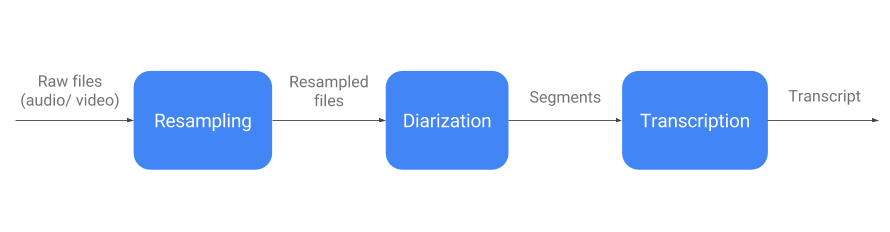
\includegraphics[width=0.9\textwidth]{../images/pipeline.png}
    \caption{Transcription processing pipeline}
\end{center}
\end{figure}

Transcription starts with the raw audio or video file, which could be
single-speaker (for example lecture recordings, Parliament speeches) or
multi-speaker (for example conversations, talk shows). The file is then resampled
to an appropriate configuration of bit rate and sample size. The resampled audio
goes through the process of speaker diarization, to separate different audio
segments (usually short) said by different speakers. These short segments are
then fed one-by-one to a transcription system; combining all the results gives
the final transcript.

For each process in the pipeline, there exists multiple solutions to perform
the task. Many of them are either public APIs or open-source; however, they exist
as ``black boxes'' --- each solution accepts input and produces output in a
specific manner. This presents a challenge in integrating multiple solutions to
realise the transcription pipeline. Additionally, given an integrated pipeline,
upgrading or changing any component could potentially break the pipeline. After
the pipeline is upgraded, there must also be a mechanism to update the
transcriptions and keep track of versions. 

This project proposes an integrated transcription system; apart from realising
the transcription pipeline, this system would be able to accommodate versioning
of all the pipeline components as well as all the transcripts. Ultimately, this
results in a simple and more efficient processing workflow for multimedia.

This project would be done in conjunction with other efforts of the Speech and
Language Technology Group in School of Computer Science and Engineering
(thereafter referred to as SLTG).

\section{Objective}

The primary objective of this project is to design a system architecture and
develop the respective system capable of performing the following tasks:

\begin{itemize}
    \item Transcription of individual audio and video files using different
    transcription solutions
    \item Transcription of multi-channel audio recording
\end{itemize}

The developed system must also have the following qualitative requirements:

\begin{itemize}
    \item Modularity --- allowing independent component operation and low coupling
    \item Extensibility --- allowing system extension to perform other related
    tasks in audio and video processing
    \item Robustness --- allowing system error recovery and process resumption
    \item Versioning --- allowing for different results with different processing
    components, and enabling evaluation of different components
    \item Logging and Reporting --- allowing developers to understand and generate
    insights to the outputs
\end{itemize}

\section{Scope}

The scope of this project is restricted to developing a system to be used in a
desktop/ laptop Ubuntu Linux environment, to perform the tasks mentioned above. A
functioning graphics user interface (GUI) is also not required.

However, the system could be modified and extended to perform other related tasks
in different environments, with a GUI\@.

\section{Project Timeline}

The project was scheduled to commence from January 2017 to October 2017. The major
milestones are as follows:

\begin{itemize}
    \item \textbf{End of January 2017:} Completion of Architectural Design
    \item \textbf{End of April 2017:} Completion of Porting of Existing Modules
    to Current System
    \item \textbf{End of September 2017:} Completion of Development of New Modules;
    Commencement of Integration Testing
    \item \textbf{End of October 2017:} Completion of Project
\end{itemize}

\section{Report Organisation}

This report is divided into four chapters:

\begin{itemize}
    \item Chapter 1 provides an introduction to the project, states its objective
    and scope and provides a timeline for completion.
    \item Chapter 2 gives a summary of the work done so far on the project
    \item Chapter 3 gives an overview to the remaining work to be done before the
    project completes.
    \item Chapter 4 concludes the report.
\end{itemize}
\chapter{Summary of Work Done}

This chapter presents a summary of the work done so far for the project. Section 2.1 covers the implemented system architecture, while Section 2.2 details the modules implemented for the integrated system.

The source code for the system has been uploaded to GitHub; GitHub also serves as the version control and issue management system for the project.

\section{System Architecture}

This section outlines the architecture of the implemented transcription system. It comprises two independent components --- \textit{modules} and \textit{data} --- each resides in its own subfolder within the system. The main system executable links these two components together; it executes \textit{procedures}, which are collections of modules in a pipeline, to complete a transcription.

The top level folder structure is as follows:

\begin{lstlisting}
    crawl/
        --raw files--
    data/
        --data files--
    modules/
        --module files--
    system.py               # system executable
    manifest.json           # system manifest
\end{lstlisting}

The whole system would be implemented in Python, using JSON as the manifest language. The components of the system architecture would be detailed below.

\subsection{Data Folders}

The data used in the system are of two types. The first type is raw data, which are unprocessed audio or video files; these files are stored under \verb|crawl/|. The second type is processed data, which are stored under \verb|data/| in a specialised folder structure:

\begin{lstlisting}
    data/
        file_id/
            raw/
                --the raw file--
            module_1/
                --output for module 1--
            module_2/
                --output for module 2--
            ...
            module_n/
                --output for module n--
            temp/
                module_1/
                    --temporary files for module 1--
                ...
\end{lstlisting}

Under this folder structure, at system startup the system executable would import the raw file from \verb|crawl/| into the \verb|data/file_id/raw/| subfolder, with the \verb|file_id| being a unique identifier. As a procedure is being executed, individual module's output files would be stored in the respective subfolder under \verb|data/file_id|, while the module's temporary files would be stored under \verb|data/file_id/temp|.

This structure allows the system to be fully modular; any module would only need to know its own folder to dump íts output, and practically any operation could be traced to the module level. Individual modules would be responsible in implementing this structure.

\subsection{Modules}

All modules in the system are placed under the subfolder \verb|modules/| according to the following folder structure:

\begin{lstlisting}
    modules/
        module_id_1/
            setup           # module setup script
            module.py       # module executable
            manifest.json   # module manifest
            --optional module data and executables--
        module_id_2/
            ...
        ...            
\end{lstlisting}

Each module has its own folder; the folder name is a module identifier in the form of \verb|module_name-version|. This allows multiple versions of a module to co-exist in the system. In each module folder there are three compulsory components --- a \verb|setup| script to setup the module and all its dependencies, a Python executable \verb|module.py| to call the module, and a manifest file in JSON format to specify the module details.

The manifest file must conform to this structure:

\begin{lstlisting}
    {
        "name": "module_name",
        "version": "module_version",
        "requires": [],
        "inputs": [],
        "outputs": []
    }
\end{lstlisting}

\verb|requires|, \verb|inputs| and \verb|outputs| are all JSON lists. \verb|requires| is a list of (optional) data files and executables required for the module's functionality; these files should be in place after running the \verb|setup| script. \verb|inputs| and \verb|outputs| are lists of subfolders under \verb|data/file_id|\footnote{See Section 2.1.1 Data Folders.} where the module would pull its input files and push its output files, respectively. In this way, the manifest file serves as a blueprint of the module to the system. This blueprint would be realised by the \verb|module.py| executable. Overall, the three compulsory components work together to ensure each module is self-contained.

\subsection{System Manifest and Executable}

The system manifest specifies system-level properties. It is a JSON file following this specification:

\begin{lstlisting}
    {
        "procedures": {
            "procedure_id_1": [],
            "procedure_id_2": [],
            ...
        },
        "file_types":{
            "audio": [],
            "video": []
        }
    }
\end{lstlisting}

\verb|file_types| would specify which file extensions are accepted by the system; only raw files of these types would be imported during runtime. The separation of \verb|audio| and \verb|video| types is used for future error-checking. \verb|procedures| as mentioned in the beginning of this chapter are pipelines of modules to perform a certain function. These procedures are specified in the manifest by unique \verb|procedure_ids|; each procedure is a list of \verb|module_ids|\footnote{See Section 2.1.2 Modules.} outlining the order of execution of the modules on the targeted audio or video file. In this way, the system manifest provides a blueprint of the whole system to the system executable; it would execute a procedure according to this flow:

\begin{itemize}
    \item Startup manifest checks --- load all module manifests and system manifest, perform error checks and eliminate all ``broken'' modules and procedures
    \item File import --- import the correct files from \verb|crawl/| into the data structure in \verb|data/|\footnote{See Section 2.1.1 Data Folders.}
    \item Pipeline --- call the modules in the procedure one-by-one in the order specified by the system manifest
\end{itemize}

Multiple procedures could be applied to one file, and multiple files could be processed in one run of the system executable.

\section{Modules Implemented}
\chapter{Summary of Work to be Done}

This chapter presents a summary of the remaining work items for the project. Section 3.1 outlines the effort to extend the implemented transcription system to handle multi-channel recordings, which is a major application focus. Section 3.2 details the necessary system improvements that needs to be implemented to realise all the objectives in Chapter 1\footnote{See Section 1.2 Objective.}.

\section{Modules and Procedures for Multi-channel Recording Transcription}

A major application focus in SLRG is multi-channel recording transcription, which is applied in a meeting room scenario. In this scenario, there are a number of speakers (denote \texttt{n}) participating in a meeting, having natural conversation with each other. Each speaker is speaking into his/ her own close-talk microphone, and there is a fix number of far-talk microphones (denote \texttt{m}) to record the entire meeting room. Despite being close to the speaker, in most meeting room environments the close-talk microphone would also capture other speakers' voice and background noise, which could impede transcription. The problem statement is, given the set of \texttt{n} close-talk and \texttt{m} far-talk recordings, perform an accurate speaker identification, and based on that derive an accurate transcription for the meeting.

The proposed workflow comprises of an initial stage, using the process of voice activity detection (VAD) across all the close- and far-talk recordings to determine which segments of the recordings are spoken by whom. All the remaining false segments will be clipped to produce \texttt{n} (hopefully pure) close-talk recordings which will be transcribed. The implementation would involve developing the VAD module and procedure.

\section{System-wide Improvements}

As of this moment, the first three qualitative objectives of the project have been relatively satisfied --- Modularity, Extensibility and Robustness. Effort would be focused in realising the two remaining objectives, which is Versioning and Logging and Reporting.

\subsection{Versioning}

The final system must be able to accommodate different module versions, and for each module version the output of such module must also be versioned. The proposed method to achieve this goal is to introduce the concept of \texttt{process}, a configuration of procedures and modules; when a module is upgraded, the associated procedure would be forked into a different procedure containing the module, and the initial process would be forked into a different process containing the new procedure. Processes should have separate folders under \texttt{data/}, resulting in this folder structure:

\begin{lstlisting}
    data/
        process_id_1/
            file_id_1/
                raw/
                module_1/
                module_2/
                ...
                module_n/
                temp/
            file_id_2/
                ...
            ...
        process_id_2/
            file_id_1/
            file_id_2/
\end{lstlisting}

The folder structure under \texttt{file\_id} remains the same, which allows for efficient evaluation of different version outputs. To specify the processes in system manifest, the following structure is proposed:

\begin{lstlisting}
    {
        "processes": {
            "process_id_1": {
                "procedure_id_1": [],
                "procedure_id_2": [],
                ...
            },
            "process_id_2": {
                "procedure_id_1": [],
                "procedure_id_2": [],
                ...
            },
            ...
        },
        ...
    }
\end{lstlisting}

To implement this structure, the system executable must be re-engineered to load the new manifest and output data to the data folders correctly. There should be minimal changes to the implemented modules, as there are no hard-coded paths that could be affected by the change in data folder structure.

\subsection{Logging and Reporting}

The final system must exhibit developer-friendly behaviours --- it must have adequate debugging logs, and it must provide an interface to report common statistics about the current data.

For logging, the system executable and modules are all using the Python standard library module \texttt{logging} to produce command-line logs, in the following format:

\begin{lstlisting}
    %(asctime)s (%(name)s | %(levelname)s) : %(message)s
\end{lstlisting}

For reporting, the proposed addition to the system executable is a reporting function to aggregate data from the data folders and provide a convenient reporting format. The usual statistics to provide are the lengths of the audio/ video streams, total processing time separated by process/ procedure, etc. Helper functionality would be incorporated accordingly to enable reporting.
\printbibliography{}
\end{document}
